\subsection{Non-linear sloshing in a rectangular container}%Ansari

Free surface oscillations of a liquid confined in a closed container (sloshing phenomenon) are an important issue when big amounts of liquid are industrially transported. The phenomenon involves two fluids that share a free surface boundary separating them, normally the density of the upper fluid is several orders of magnitude less than the bottom one. This phenomenon has proven of great interest due to the fact that violent impacts of the fluid can affect the structural integrity of the container.

For studied cases in this section, the sloshing phenomenon is produced by a horizontal harmonic excitation $x = a_h (\sin \omega_h t)$, where $a_h$ is the excitation amplitude and $\omega_h$ is the excitation frequency of the rectangular tank where the two fluid phases are contained. The tank is divided in two parts, the bottom part is water with a density of $\rho_{I} = 1000 [kg/m^3]$ and the top part contains a fluid with different densities $\rho_{II} = 1.3, 50, 200, 800 [kg/m^3]$, depending on the studied case. The dimensions of the tank are $a$(width) by $b$(height) and the initial free surface is at height $h$ from the bottom of the tank, see Figure \ref{fg:ansari-config}. The free surface starts the simulation as a horizontal line and is subsequently deformed by the tank excitation and the flow dynamics.

\begin{figure}[H]
  \begin{center}
      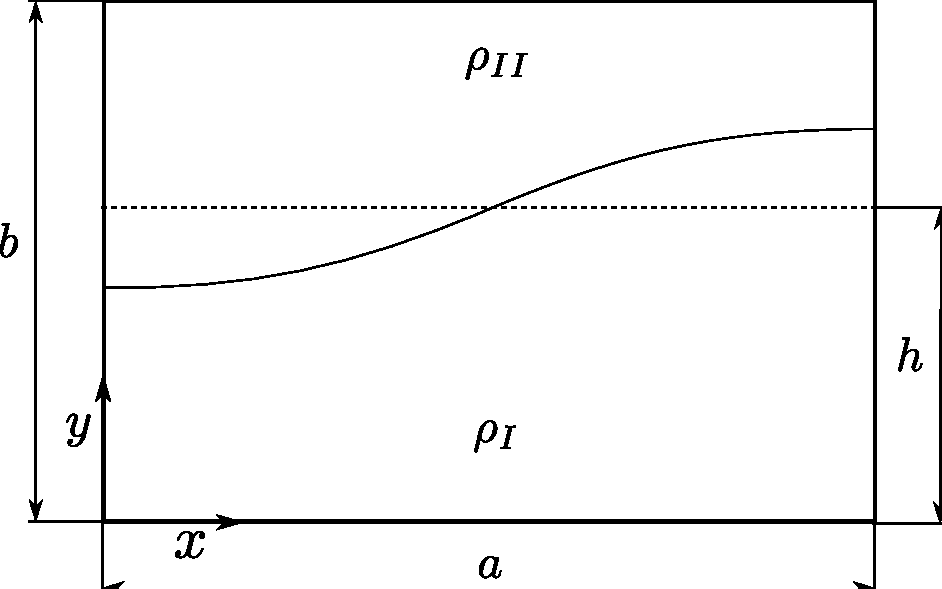
\includegraphics[width=.6\columnwidth]{images/ansari_config.pdf}
  \end{center}
  \caption{\label{fg:ansari-config} Configuration of the Non-linear sloshing in a rectangular container case. Initial condition is represented by dashed lines. Continuous line represents the position of the free-surface for a certain time.}
\end{figure}

For the different cases in this report, a 2D rectangular tank $a=1.0[m]$ width by $b=1.0[m]$ height is used. The initial height of the interface is $h=0.5[m]$ and the lateral excitation applied is $x=0.05\sin(3t)$. The simulations were performed considering the
flow as laminar and non-viscous, hence no turbulence model was used and slip boundary conditions are taken. Density was modified according to the considered ratios $\sigma=\frac{\rho{II}}{\rho{I}}$. A two dimensional Cartesian mesh of $450\times225$, splitted into triangles, has been used in all cases.

Reference results for this case are taken from \cite{Goni13} which uses the codes STARCCM+ and \OF to obtain numerical solutions and reports the free surface displacement on the left wall of the container. Those simulations use the same grid as presented above, but, in order to avoid numerical instabilities, they limit the $CFL$ number to $CFL_{max}=0.5$ then they use $\Delta t \approx 0.001$. In PFEM-2 simulations do not exist that restriction then $\Delta t$ is fixed to $0.01$, reaching $CFL_{max}\approx5$. 
Figure \ref{fg:ansari-results} presents the free surface displacement reported on the left wall of the container for different density ratios. For each one of them, PFEM-2 simulations shows a good agreement with reference solutions, further more considering that the time step used is around ten times bigger than the used in \cite{Goni13}.


  \begin{figure}[h]
  \centering
    \subfloat[]{
	  \label{fg:ansari-1}         %% Etiqueta para la primera subfigura
	  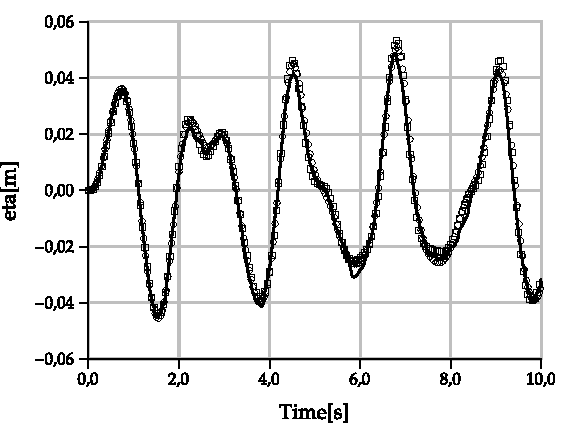
\includegraphics[width=.49\columnwidth]{images/ansari_1.pdf}
    }
    %%----segunda subfigura----
    \subfloat[]{
	  \label{fg:ansari-2}         %% Etiqueta para la segunda subfigura
	  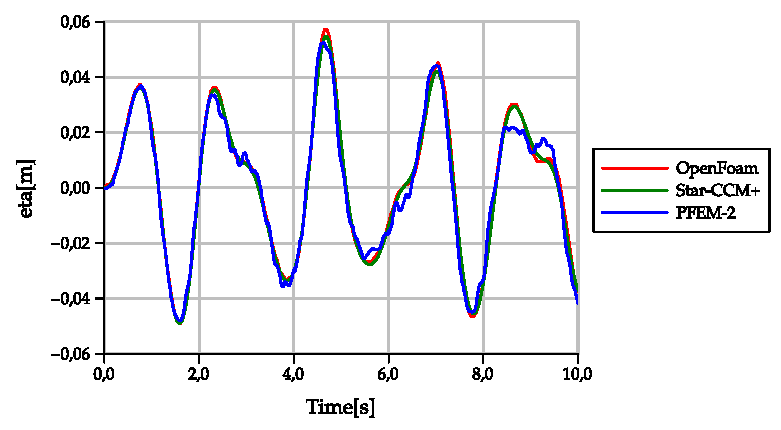
\includegraphics[width=.49\columnwidth]{images/ansari_2.pdf}
    } \\
    \subfloat[]{
	  \label{fg:ansari-3}         %% Etiqueta para la primera subfigura
	  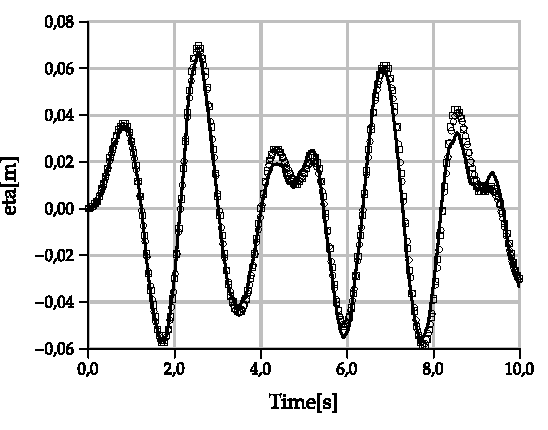
\includegraphics[width=.49\columnwidth]{images/ansari_3.pdf}
    }
    %%----segunda subfigura----
    \subfloat[]{
	  \label{fg:ansari-4}         %% Etiqueta para la segunda subfigura
	  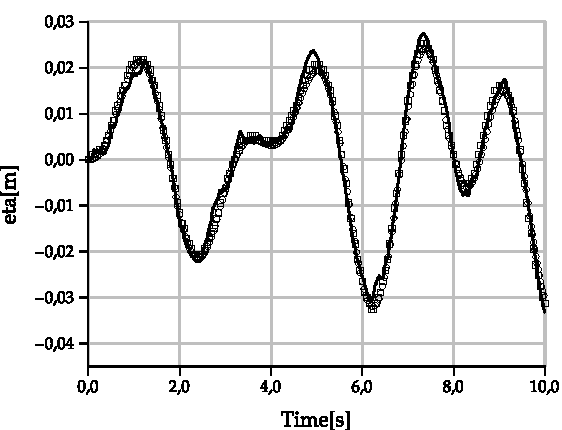
\includegraphics[width=.49\columnwidth]{images/ansari_4.pdf}
    }
   \caption{Level of height on the left wall for a two phase flow for different density ratios. Figure \ref{fg:ansari-1}: $\sigma=0.0013$, Figure \ref{fg:ansari-2}: $\sigma=0.05$, Figure \ref{fg:ansari-3}: $\sigma=0.2$ and Figure \ref{fg:ansari-4}: $\sigma=0.8$. References:\ \Circle \ STARCCM, \Square \ OpenFOAM and filled line PFEM-2.}
   \label{fg:ansari-results}                %% Etiqueta para la figura entera
\end{figure}

\clearpage
